\section{基准测试}
\subsection{概览}
选择的图像分类模型被多平台测试为TensorFlow社区创建一个参考点。在\href{https://www.tensorflow.org/performance/benchmarks#methodology}{Methodology }章节详细描述了测试如何执行和连接到使用脚本。
\subsection{图形分类模型的结果}
InceptionV3(\href{https://arxiv.org/abs/1512.00567}{arXiv:1512.00567)}),ResNet-50(\href{https://arxiv.org/abs/1512.03385}{arXiv:1512.03385}),ResNet-152(\href{https://arxiv.org/abs/1512.03385}{arXiv:1512.03385}),VGG16(\href{https://arxiv.org/abs/1409.1556}{arXiv:1409.1556})和\href{http://papers.nips.cc/paper/4824-imagenet-classification-with-deep-convolutional-neural-networks.pdf}{AlexNet}使用\href{http://www.image-net.org/}{ImageNet}数据集。测试运行在Google Compute Engine,Amazon Elastic Compute Cloud(Amazon EC2),和NVIDIA DGX-1。多数测试运行在合成和真实数据上。测试合成数据通过使用tf.Variable设置相同的形状作为ImageNet模型的数据期望。我们相信在一个平台的基准测试上它是很有用的。这载入基础的永健和实际训练准备数据的框架测试。我们结合合成数据移除磁盘I/O作为变量设置baseline。真真的数据用于验证TensorFlow输入pipeline和基础的磁盘I/O在计算单元上是饱和。
\subsection{在NVIDIA DGX-1(NVIDIA Tesla P100)}
\begin{figure}[H]
	\centering
	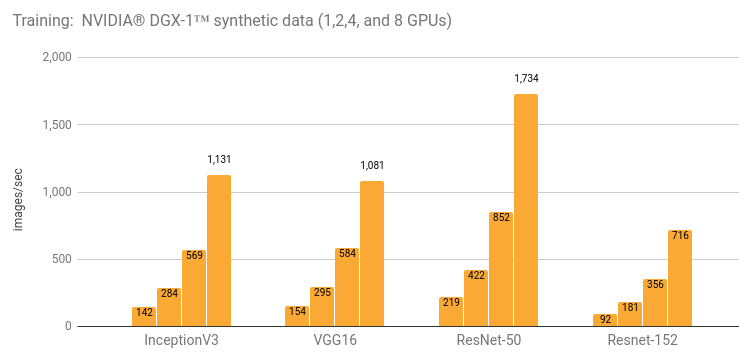
\includegraphics[scale=0.5]{perf_summary_p100_single_server.png}
\end{figure}
详细的额外的结果在\href{https://www.tensorflow.org/performance/benchmarks#details_for_nvidia_dgx-1tm_nvidia_tesla_p100}{Details for NVIDIA® DGX-1 (NVIDIA TeslaP100)}
\begin{figure}[H]
	\centering
	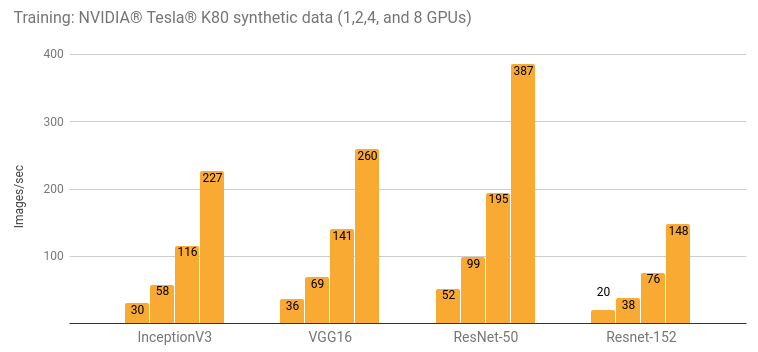
\includegraphics[scale=0.5]{perf_summary_k80_single_server.png}
\end{figure}
详细的额外的结果在\href{https://www.tensorflow.org/performance/benchmarks#details_for_google_compute_engine_nvidia_tesla_k80}{Details for Google Compute Engine (NVIDIA Tesla K80) }和\href{https://www.tensorflow.org/performance/benchmarks#details_for_amazon_ec2_nvidia_tesla_k80}{ Details for Amazon EC2 (NVIDIA Tesla K80) }
\subsection{用Tesla K80分布式的训练}
\begin{figure}[H]
	\centering
	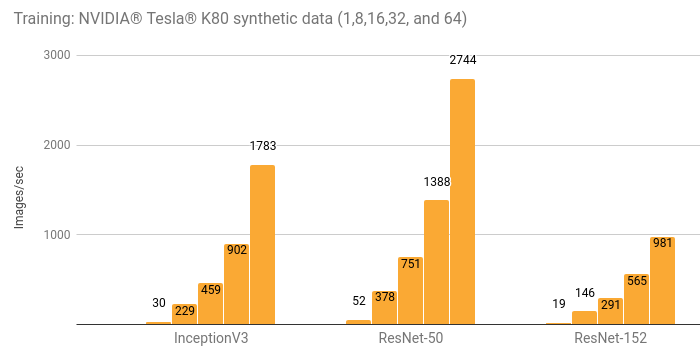
\includegraphics[scale=0.5]{perf_summary_k80_aws_distributed.png}
\end{figure}
详细的信息在\nameref{subsec:1}
\subsection{结合真是数据训练比较}
\begin{figure}[H]
	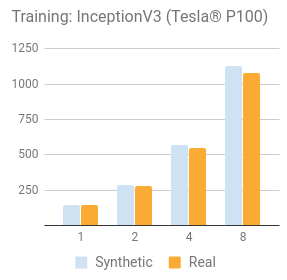
\includegraphics[scale=0.5]{perf_summary_p100_data_compare_inceptionv3}
	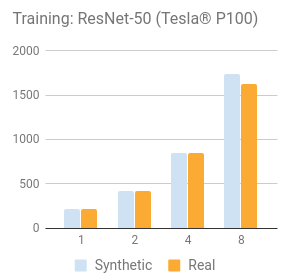
\includegraphics[scale=0.5]{perf_summary_p100_data_compare_resnet50}
\end{figure}
NVIDIA Tesla K80
\begin{figure}[H]
	\centering
	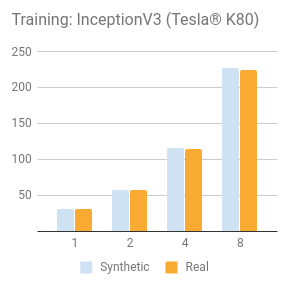
\includegraphics[scale=0.5]{perf_summary_k80_data_compare_inceptionv3.png}
	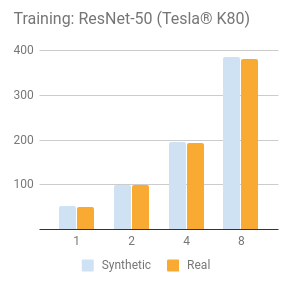
\includegraphics[scale=0.5]{perf_summary_k80_data_compare_resnet50.png}
\end{figure}
\subsection{详细的NVIDIA DGX-1(NVIDIA Tesla P100)}
\textbf{环境}\newline
\begin{itemize}
	\item 实例类型:NVIDIA DGX-1
	\item GPU:8x NVIDIA Tesla P100
	\item OS:通过Docker特使运行Ubuntu 16.0.4 LTS 
	\item CUDA/cuDNN"8.0/5.1
	\item TensorFlow GitHub b1e174e
	\item Benchmark GitHub hash:9165a70
	\item 构建命令:\lstinline[language=Bash]{bazel build -c opt --copt=-march="haswell" --config=cuda //tensorflow/tools/pip_package:build_pip_package}
	\item Disk:本地SSD
	\item Dataset:ImageNet
	\item Test Data:2017五月
\end{itemize}
用于模型的批大小和优化器在下表。另外在表中的批大小,Inception V3,ResNet-50,ResNet152和VGG16用于在批大小为32上测试,这些值在其他的结果章节:
\begin{table}[H]
	\begin{tabular}{|c|c|c|c|c|c|}
		选项&Inception v3&ResNet-50&ResNet-152&AlexNet&VGG16\\
		每个GPU批的大小&64&64&64&512&64\\
		优化器&sgd&sgd&sgd&sgd&sgd\\
	\end{tabular}
\end{table}
为每个模型配置:
\begin{table}[H]
	\begin{tabular}{|c|c|c|}
	模型&变量更新&本地变量设备\\
		InceptionV3 &参数服务器&cpu\\
		ResNet50 &参数服务器&cpu\\
		ResNet152 &参数服务器&cpu\\
		AlexNet &参数服务器&cpu\\
		VGG16 &参数服务器&cpu\\
	\end{tabular}
\end{table}
结果:
\begin{figure}[H]
	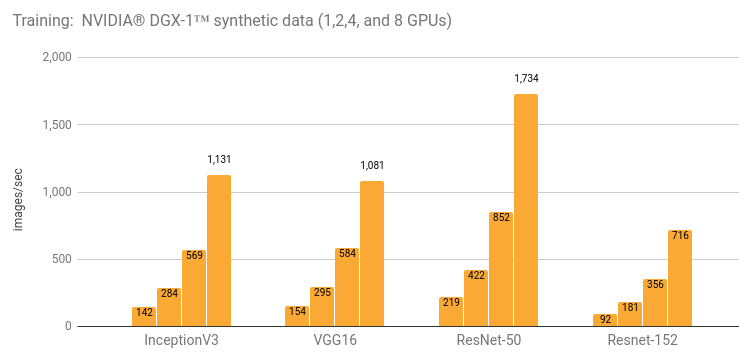
\includegraphics[scale=0.5]{perf_summary_p100_single_server.png}
	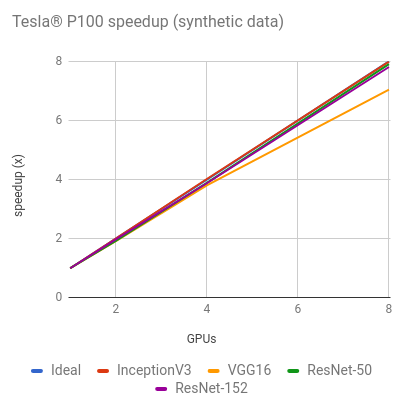
\includegraphics[scale=0.5]{perf_dgx1_synth_p100_single_server_scaling.png}
\end{figure}
训练聚合数据
\begin{table}H[]
	\begin{tabular}{|c|c|c|c|c|c|}
		GPUs	&InceptionV3	&ResNet-50	&ResNet-152	&AlexNet	&VGG16\\
		1	&142	&219	&91.8	&2987	&154\\
		2	&284	&422	&181	&5658	&295\\
		4	&569	&852	&356	&10509	&584\\
		8	&1131	&1734	&716	&17822	&1081\\
	\end{tabular}
\end{table}
训练真是数据
\begin{table}[H]
	\begin{tabular}{|c|c|c|c|c|c|}
		GPUs	&InceptionV3	&ResNet-50	&ResNet-152	&AlexNet	&VGG16\\
		1	&142	&218	&91.4	&2890	&154\\
		2	&278	&425	&179	&4448	&284\\
		4	&551	&853	&359	&7105	&534\\
		8	&1079	&1630	&708	&N/A	&898\\
	\end{tabular}
\end{table}
在8GPUs结合真实数据训练AlexNet从图上包含上面的表格最大化输入pipeline。
其他的结果

下面的结果每批32
\textbf{训练综合数据}
\begin{table}[H]
	\begin{tabular}{|c|c|c|c|c|}
		GPUs	&InceptionV3	&ResNet-50	&ResNet-152	&VGG16\\
		1	&128	&195	&82.7	&144\\
		2	&259	&368	&160	&281\\
		4	&520	&768	&317	&549\\
		8	&995	&1485	&632	&820\\
	\end{tabular}
\end{table}

训练真实数据
\begin{table}
	\begin{tabular}{|c|c|c|c|c|}
		GPUs	&InceptionV3	&ResNet-50	&ResNet-152	&VGG16\\
		1	&130	&193	&82.4	&144\\
		2	&257	&369	&159	&253\\
		4	&507	&760	&317	&457\\
		8	&966	&1410	&609	&690\\
	\end{tabular}
\end{table}
在Google Compute Engine上详情(NVIDIA Tesla K80)
\begin{itemize}
	\item  实例类型:n1-standard-32-k80x8
	\item  GPU:8 NVIDIA Tesla K80
	\item OS Ubuntu 16.04 LTS 
	\item CUDA/cuDNN:8.0/5.1
	\item TensorFlow GitHub hash:b1e174e
	\item Benchmark Github hash:9165a70
	\item 构建命令\lstinline[language=Bash]{bazel build -c opt --copt=-march="haswell" --config=cuda //tensorflow/tools/pip_package:build_pip_package}
	\item Disk:1.7TB共享SSD永久磁盘
	\item Dataset:ImageNet 
	\item Test Data:2017 5月
\end{itemize}
每个模型的批大小和优化器在下表中。另外批大小列在表格,InceptionV3和ResNet-50被测试一个batch为32,这些结果在其他章节。
\begin{table}[H]
	\begin{tabular}{|c|c|c|c|c|}
		Options	&InceptionV3	&ResNet-50	&ResNet-152	&AlexNet	&VGG16\\
		Batch size per GPU	&64	&64	&32	&512	&32\\
		Optimizer	&sgd	&sgd	&sgd	&sgd	&sgd\\
	\end{tabular}
\end{table}
这配置用于每个模型variable\_update等于parameter\_server和local\_parameter\_device等于cpu。
\textbf{结果}\\
\begin{figure}[H]
	\centering
	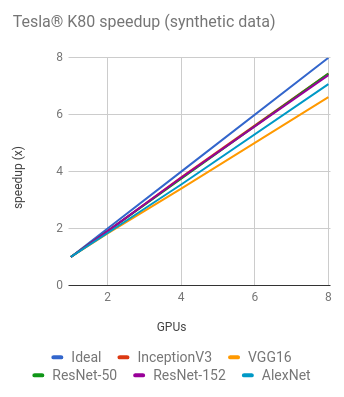
\includegraphics[scale=0.5]{perf_gce_synth_k80_single_server_scaling.png}
	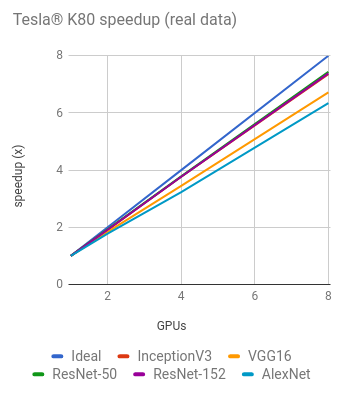
\includegraphics[scale=0.5]{perf_gce_real_k80_single_server_scaling.png}
\end{figure}
\begin{table}[H]
	\begin{tabular}{|c|c|c|c|c|}
		GPUs	&InceptionV3	&ResNet-50	&ResNet-152	&AlexNet	&VGG16\\
		1	&30.5	&51.9	&20.0	&656	&35.4\\
		2	&57.8	&99.0	&38.2	&1209	&64.8\\
		4	&116	&195	&75.8	&2328	&120\\
		8	&227	&387	&148	&4640	&234\\
	\end{tabular}
	\caption{Training synthetic data}
\end{table}
\begin{table}[H]
	\begin{tabular}{|c|c|c|c|c|c|}
		GPUs	&InceptionV3	&ResNet-50	&ResNet-152	&AlexNet	&VGG16\\
		1	&30.6	&51.2	&20.0	&639	&34.2\\
		2	&58.4	&98.8	&38.3	&1136	&62.9\\
		4	&115	&194	&75.4	&2067	&118\\
		8	&225	&381	&148	&4056	&230\\
	\end{tabular}
	\caption{训练真实数据}
\end{table}
\begin{table}[H]
	\begin{tabular}{|c|c|c|}
		GPUs	&InceptionV3 (batch size 32)	&ResNet-50 (batch size 32)\\
		1	&29.3	&49.5\\
		2	&55.0	&95.4\\
		4	&109	&183\\
		8	&216	&362\\
	\end{tabular}
	\caption{Training real data}
\end{table}
\subsection{Amazon Ec2详情(NVIDIA Tesla K80)}
环境
\begin{itemize}
	\item 实例类型:p2.8xlarge
	\item GPU:8x NVIDIA Tesla K80
	\item OS:Ubuntu16.0.4 LTS 
	\item CUDA/cuDNN:8.0/5.1
	\item TensorFlow Github hash:b1e174e
	\item Benchmark GitHub hash:9165a70
	\item 构建命令\lstinline[language=Bash]{bazel build -c opt --copt=-march="haswell" --config=cuda //tensorflow/tools/pip_package:build_pip_package}
	\item Disk:1TB Amazon EFS(brush 100MiB/sec for 12 hours,continous 50 MiB/sec)
	\item Dataset:ImageNet 
	\item TestData:2017 5月
\end{itemize}
用于每个模型的Batch size和优化器在下表。另外batch size列出在表格中,InceptionV3和ResNet-50用于在batch为32上测试。这些结果在其它章节
\begin{table}
\begin{tabular}{|c|c|c|c|c|}
	Options	InceptionV3	&ResNet-50	&ResNet-152	&AlexNet	&VGG16\\
	Batch size per GPU	&64	&64	&32	&512	&32\\
	Optimizer	&sgd	&sgd	&sgd	&sgd	&sgd\\
\end{tabular}
\end{table}
用于每个模型的配置
\begin{table}[H]
	\begin{tabular}{|c|c|c|}
		Model	&variable\_update	&local\_parameter\_device\\
		InceptionV3	&parameter\_server	&cpu\\
		ResNet-50	&replicated (without NCCL)	&gpu\\
		ResNet-152	&replicated (without NCCL)	&gpu\\
		AlexNet	&parameter\_server	&gpu\\
		VGG16	&parameter\_server	&GPUs \\
	\end{tabular}
\end{table}
 结果
 \begin{figure}[H]
	 \centering
	 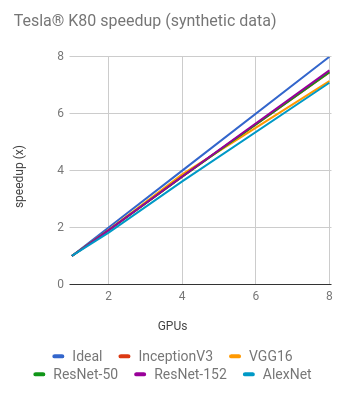
\includegraphics[scale=0.5]{perf_aws_synth_k80_single_server_scaling.png}
	 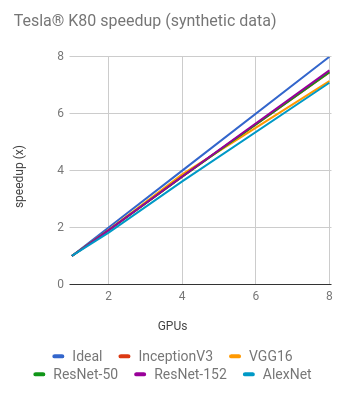
\includegraphics[scale=0.5]{perf_aws_synth_k80_single_server_scaling.png}
 \end{figure}
 \begin{table}[H]
	\begin{tabular}{|c|c|c|c|c|c|}
		GPUs	&InceptionV3	&ResNet-50	&ResNet-152	&AlexNet	&VGG16\\
		1	&30.8	&51.5	&19.7	&684	&36.3\\
		2	&58.7	&98.0	&37.6	&1244	&69.4\\
		4	&117	&195	&74.9	&2479	&141\\
		8	&230	&384	&149	&4853	&260\\
	\end{tabular}
	 \caption{Training synthetic data}
\end{table}
 \begin{table}[H]
	 \begin{tabular}{|c|c|c|c|c|c|}
		 GPUs	&InceptionV3	&ResNet-50	&ResNet-152	&AlexNet	&VGG16\\
		 1	&30.5	&51.3	&19.7	&674	&36.3\\
		 2	&59.0	&94.9	&38.2	&1227	&67.5\\
		 4	&118	&188	&75.2	&2201	&136\\
		 8	&228	&373	&149	&N/A	&242\\
	 \end{tabular}
 \end{table}
 结合8GPU从图上和表格训练真实数据因为我们的RFS设置没有提供足够的吞吐量。
 
 其他的结果
 \begin{table}[H]
	\begin{tabular}{|c|c|c|}
		GPUs	&InceptionV3 (batch size 32)	&ResNet-50 (batch size 32)\\
		1	&29.9	&49.0\\
		2	&57.5	&94.1\\
		4	&114	&184\\
		8	&216	&355\\
	\end{tabular}
	 \caption{Training synthetic data}
\end{table}
 \begin{table}[H]
	\begin{tabular}{|c|c|c|}
		GPUs	&InceptionV3 (batch size 32)	&ResNet-50 (batch size 32)\\
		1	&30.0	&49.1\\
		2	&57.5	&95.1\\
		4	&113	&185\\
		8	&212	&353\\
	\end{tabular}
	 \caption{Training real data}
\end{table}
 \subsection{在Amazon EC2上(NVIDIA Tesla K80)}
 \begin{itemize}
	 \item Instance type: p2.8xlarge
         \item GPU: 8x NVIDIA® Tesla® K80
	 \item  OS: Ubuntu 16.04 LTS
	\item 	 CUDA / cuDNN: 8.0 / 5.1
	\item 	 TensorFlow GitHub hash: b1e174e
	\item 	 Benchmark GitHub hash: 9165a70
	\item 	\lstinline[language=Bash]{} Build Command: bazel build -c opt --copt=-march="haswell" --config=cuda //tensorflow/tools/pip_package:build_pip_package}
	\item 	 Disk: 1.0 TB EFS (burst 100 MB/sec for 12 hours, continuous 50 MB/sec)
	\item 	 DataSet: ImageNet
	\item	 Test Date: May 2017
 \end{itemize}
 用于测试的批和优化器在下表。另外批大小在表格中,InceptionV3和ResNet-50用于在批大小为32上测试。这结果在其它章节。
 \begin{table}[H]
	 \begin{tabular}{|c|c|c|c|c|}
		 Options	&InceptionV3	&ResNet-50	&ResNet-152\\
		 Batch size per GPU	&64	&64	&32\\
		 Optimizer	&sgd	&sgd	&sgd\\

	 \end{tabular}
 \end{table}
 用于每个模型的配置

\begin{table}
	\begin{tabular}{|c|c|c|c|}
		Model	&variable\_update	&local\_parameter\_device	&cross\_replica\_sync\\
		InceptionV3	&distributed\_replicated	&n/a	&True\\
		ResNet-50	&distributed\_replicated	&n/a	&True\\
		ResNet-152	&distributed\_replicated	&n/a	&True\\
	\end{tabular}
\end{table}
为了简化服务器设置,EC2实例(p2.8xlarge)运行在worker服务器上也运行在参数服务器上。参数服务器数量和worker服务器用:
\begin{itemize}
		\item InceptionV3:8实例/参数服务器
		\item ResNet50:(批大小为32)8实例/4参数服务器
		\item ResNet-152:8shili /4参数服务器
\end{itemize}
 结果
 \begin{figure}[H]
	 \centering
	 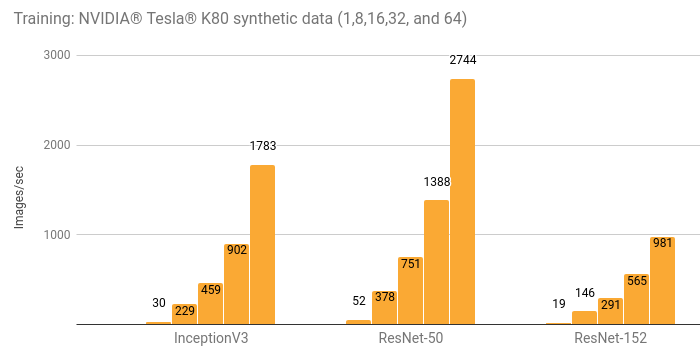
\includegraphics[scale=0.5]{perf_summary_k80_aws_distributed.png}
 \end{figure}
 \begin{figure}[H]
	 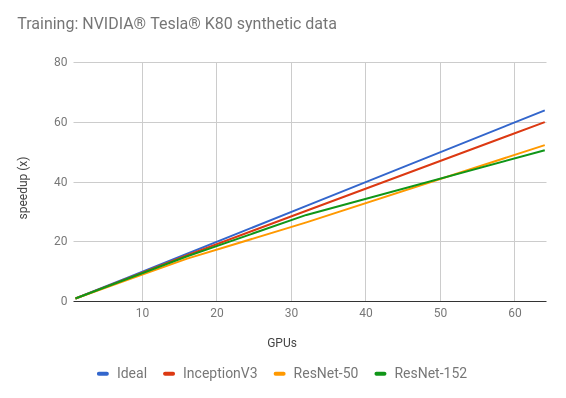
\includegraphics[scale=0.5]{perf_aws_synth_k80_distributed_scaling.png}
 \end{figure}
 \begin{table}
	 \begin{tabular}{|c|c|c|c|}
		 GPUs	&InceptionV3	&ResNet-50	&ResNet-152\\
		 1	&29.7	&52.4	&19.4\\
		 8	&229	&378	&146\\
		 16	&459	&751	&291\\
		 32	&902	&1388	&565\\
		 64	&1783	&2744	&981\\
	 \end{tabular}
 \end{table}
 其他结果
 \begin{figure}[H]
	 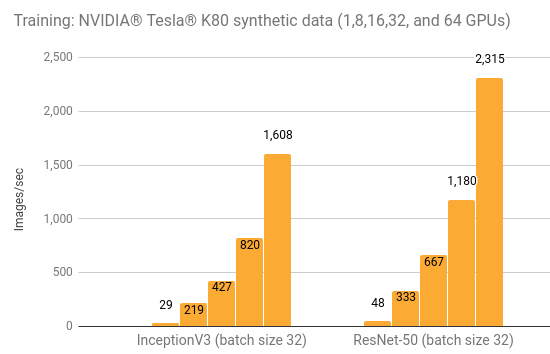
\includegraphics[scale=0.5]{perf_aws_synth_k80_multi_server_batch32.png}
 \end{figure}
 \begin{table}[H]
	 \begin{tabular}{|c|c|c|}
		 GPUs	&InceptionV3 (batch size 32)	&ResNet-50 (batch size 32)\\
		 1	&29.2	&48.4\\
		 8	&219	&333\\
		 16	&427	&667\\
		 32	&820	&1180\\
		 64	&1608	&2315\\
	 \end{tabular}
 \end{table}
 \subsection{方法论}
 这个\href{https://github.com/tensorflow/benchmarks/tree/master/scripts/tf_cnn_benchmarks}{脚本}运行在多个平台生成上面的结果。\href{https://www.tensorflow.org/performance/performance_models}{High-Performance Models}如何执行脚本的例子的详细技术在脚本中。

 为了创建结果可重复,没个测试运行5次然后时间被平均。GPU运行在默认给定的平台。对于NVIDIA Tesla K80这意味着让\href{https://devblogs.nvidia.com/parallelforall/increase-performance-gpu-boost-k80-autoboost/}{GPU Boose},10warmup步被做然后下一个100步被平均。
